\documentclass[10pt]{article}
\usepackage{lettrine}
\usepackage{titletoc}
\usepackage{indentfirst}
\usepackage{xcolor}
\usepackage{float}
\definecolor{lakeblue}{rgb}{0,0.55,0.71}
\usepackage{multicol}
\setlength{\columnsep}{0.4in}
\usepackage{amsmath}
\usepackage{geometry}
\geometry{left=0.75in, right=0.75in, top=0.8in, bottom=1in}
\usepackage[dvips]{graphicx}
\usepackage{wrapfig}
\graphicspath{{eps/}}
\DeclareGraphicsExtensions{.eps}
\usepackage{fancyhdr}
\pagestyle{fancy}
\lfoot{\footnotesize\textcolor{lakeblue}{PROJECT \& RESEARCH EXPERIENCE}}
\rfoot{\footnotesize\textcolor{lakeblue}{\thepage}}
\cfoot{}
\lhead{}
\rhead{}

\begin{document}
\newpage

\begin{minipage}[t]{1\linewidth}
\renewcommand{\contentsname}{\textcolor{lakeblue}{Youzheng Chen's Project \& Research Experience}}
\setlength{\baselineskip}{26pt}
\tableofcontents
\end{minipage}
\thispagestyle{empty}
\newpage
\setcounter{page}{1}
\begin{center}
\section*{\textcolor{lakeblue}{ECHelper - A Mobile Medical System}}
\addcontentsline{toc}{section}{ECHelper - A Mobile Medical System}
\end{center}

\noindent
\begin{minipage}[t]{0.77\linewidth}
\vspace{-0.5in}
\em \lettrine[lines=2, loversize=0.35,lraise=0.07,findent=7pt,nindent=0pt]{\textit{E}}{}CHelper is the project three friends and I made for Microsoft Imagine Cup Software Challenge, achieving the high-efficient data communication between patients and doctors, providing first aid to the cardiac patients.
\end{minipage}
\hfill
\begin{minipage}[t]{0.2\linewidth}

\includegraphics[width=1\linewidth]{ECHelper}
\end{minipage}
 
\begin{multicols}{2}

\subsection*{\centerline{Inspiration}}
\addcontentsline{toc}{subsection}{Inspiration}

As we grows older, many of us will have great risks in getting heart attack, but not all the people can realize their disease in time, especially in their early life. ``The Sopranos" actor James Gandolfini, 51, died of an apparent heart attack. Sage Stallone, son of actor Sylvester Stallone, died of atherosclerosis, a condition that brought on a heart attack at the age of 36. Besides, because of the short period of disease, many patients cannot go to hospital in time for being examined, which prevent doctors from making diagnoses.

However, currently there are few products concerning about the prevention of heart disease, since treatment is the most important topic in this area. We often ignore some subtle changes in our body when working hard and devoting ourselves to scientific research. Think about our relatives and friends, if some of them have lost their lives in heart attack but even unaware it, we cannot help ourselves feeling sorrow and loss.

The world is entering into the senior age. No matter what the seniors are doing, they deserve our atmost care for not only their immense love for us but also we ourselves are becoming them one day. An efficient way to monitor and treat the disease is extremely necessary for our society.  ECHelper is designed to assist patients by calling the family doctors in an emergency or provide regular monitor for patients.

\subsection*{\centerline{Market Analysis}}
\addcontentsline{toc}{subsection}{Market Analysis}

According to a report of WHO on September 29th, 2011, cardiovascular disease is the first killer in the world. There are an estimated 17.3 million people died from CVDs in 2008. By 2030, almost 23.6 million people will die from CVDs. 

Our survey (whose data comes from Sina Weibo and Tencent Weibo) indicates that more than half of doctor-related people register as authentication doctor for better helping people in their leisure time.

\begin{figure}[H]
\centering
\includegraphics[width=0.7\linewidth]{Screenshot}
\end{figure}

\subsection*{\centerline{Architecture \& Technology}}
\addcontentsline{toc}{subsection}{Architecture \& Technology}

The architecture of the solution is shown to the right. Model-View-ViewModel (MVVM) pattern is applied in the design of two clients (patients' \& doctors'). All the clients communicate via WCF RIA Service, which is hosted in Windows Azure. In addition, a ECG Sensor can be used for transferring patients� monitoring data to a Windows 8 Metro Style Application. A custom Windows Service is introduced for driver implementation in Virtual Serial Port.

ECG data will be recorded in byte-stream file and synchronized to Blob in Azure. Shared Access Signature is introduced for improvement of the security of private data.

For the purpose of improvement of user experience, we avail ourselves of Access Control Service to integrate identity federation and single sign-on.

\begin{figure}[H]
\centering
\includegraphics[width=1\linewidth]{ArchE}
\end{figure}

\subsection*{\centerline{Scenarios \& Vision}}
\addcontentsline{toc}{subsection}{Scenarios \& Vision}

In {\em Outpatient Service}, patients can obtain help from their family doctors by exchange monitoring data. In {\em Emergency Service}, patients can get the first aid from doctors nearby with the help of GPS. In other scenarios, for instance, doctors should register in an official way, history of medical record can only be reviewed by corresponding doctors, etc.

Our aim is to build a new medical treatment pattern between patients and doctors. It is a new direction to make full use of medical resources, relieving the seriousness of seeing doctors in developing countries, also providing more convenient routes for community medical service in developed countries.

\end{multicols}

\begin{center}
\section*{\textcolor{lakeblue}{GryffinAS - Access Control System of Intelligent Apartment}}
\addcontentsline{toc}{section}{GryffinAS - Access Control System of Intelligent Apartment}
\end{center}

\noindent
\begin{minipage}[t]{0.2\linewidth}

\includegraphics[width=1\linewidth]{GryffinAS}
\end{minipage}
\hfill
\begin{minipage}[t]{0.77\linewidth}
\vspace{-0.5in}
\em \lettrine[lines=2, loversize=0.35,lraise=0.07,findent=7pt,nindent=0pt]{\textit{S}}{}ponsored by Hongfu Group, GryffinAS is my graduate project in Beijing Univ. Post. \& Telecom., achieving Access Control Function and Call Center Function for the elderly in intelligent apartment of Hot Spring Leisure City.
\end{minipage}

\begin{multicols}{2}

\subsection*{\centerline{Motivation}}
\addcontentsline{toc}{subsection}{Motivation}

The current system of Intelligent Apartment for elderly was out of scope. My research here focused on the potencial requirement and perspective improvement. When I considered how to match the requirement of Access Control System perfectly, I proposed a widespread mechanism--Call Transfer--to replace the video conference architecture and revised SIP (Session Initiation Protocol) workflow. In addition, I also suggested the Interactive Voice Response (IVR) system to cut down the demand of support staffs. Taking graduate design as an opportunity, this is a perspective exploration on functions of access control system and call center.

\subsection*{\centerline{Requirement Analysis}}
\addcontentsline{toc}{subsection}{Requirement Analysis}

This system mainly serves the visitors of Intelligent Apartment. When the visitors standing at the door, they can communicate with this system for the help of finding their relatives or friends. Three ways are described below:

\begin{enumerate}
\item If visitor is familiar with the elderly, they can directly call him via the SIP terminal.
\item If visitor can only remember some information about the elderly, the self-service terminal can be used for interactive voice response (IVR).
\item If visitor cannot explicitly describe the details about the elderly, the terminal can transfer the call to the apartment administrator for help.
\end{enumerate}

\begin{figure}[H]
\centering
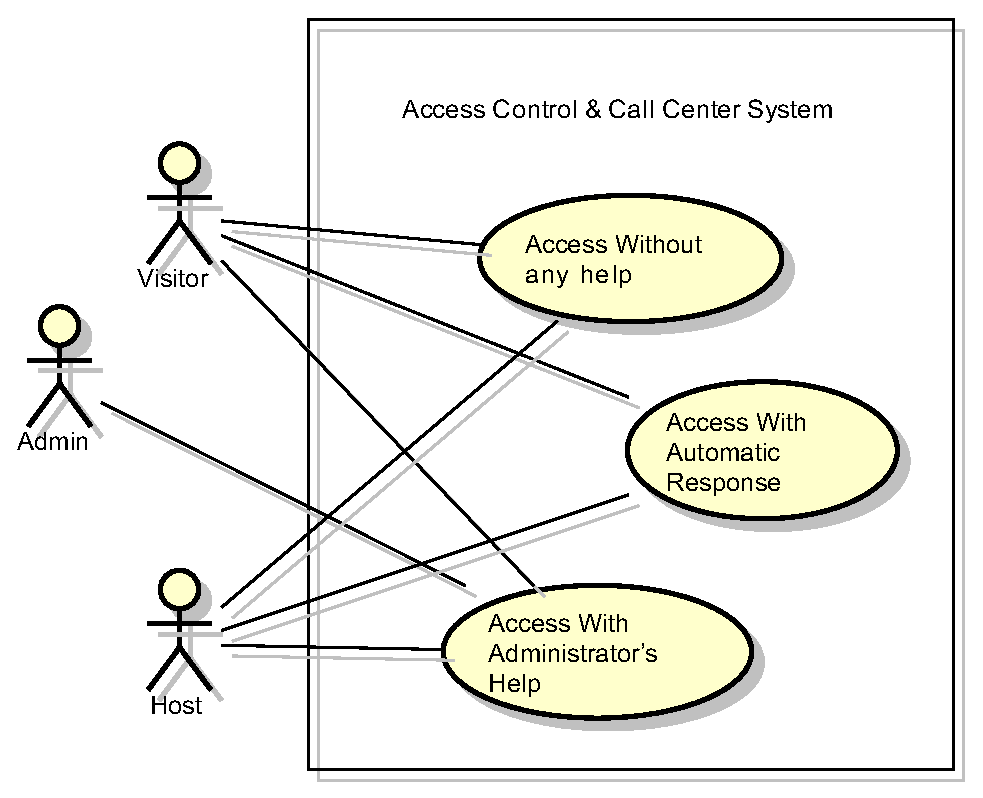
\includegraphics[width=0.65\linewidth]{UseCase}
\end{figure}

\subsection*{\centerline{Design \& Implementation}}
\addcontentsline{toc}{subsection}{Design \& Implementation}

The solution includes six separate parts: IMS Client, IMS Application Server (AS), IMS Core, Web Client, Web Server and Information Database. Gryffin-AS is focus on IMS Application Server, achieving IVR Function and Call Manipulation.

Based on JAIN SLEE, I primarily designed the business logic of the AS, serving as signal proxy between Client and Media Server (MS). According to the customized script on business logic, GryffinAS can provide corresponding media service for its clients.

\begin{figure}[H]
\centering
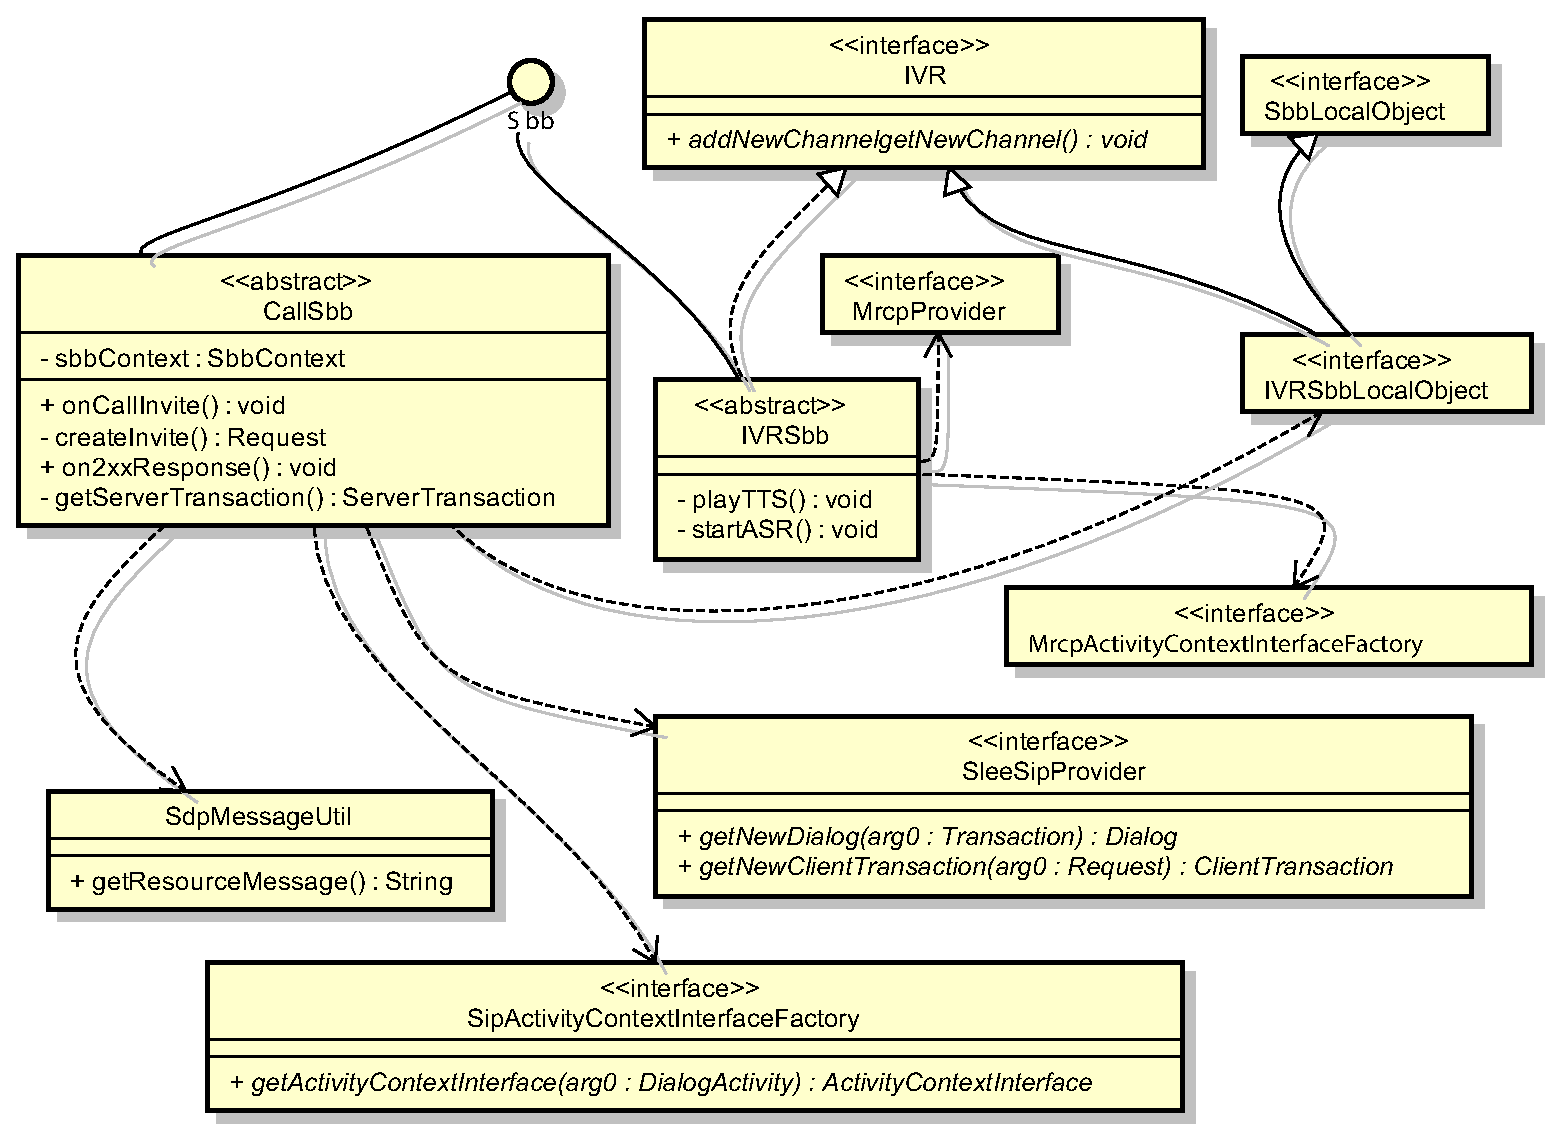
\includegraphics[width=1\linewidth]{Class}
\end{figure}

The primary work in this project is to design the SLEE-based Service Building Blocks (SBBs) and MRCP4J-based Resource Adaptor (RA). In terms of the design of SBBs, it involves {\em CallSbb} and {\em IVRSbb}, respectively handling SIP messages and Media Resource Control Protocol (MRCP) messages.

When it comes to RA, I designed the interface and implementation of resource adaptor strictly follow the design patterns of JAIN SLEE. 

When considering the aspect of implementation, three key jobs has been completed:

\begin{enumerate}
\item Message interpretation and package encapsulation are well-developed for adding media resource control signal.
\item The design of MRCP RA has considered interface definition for SBB for controlling media resources, including speech recognition \& synthesis.
\end{enumerate}

\subsection*{\centerline{Vision}}
\addcontentsline{toc}{subsection}{Vision}

With social wealth increasing, apartments for elderly have been developing and perfecting. More and more old people enjoy leisure and recreation here; They access healthcare of good quality with well-equipped facilities and elegant environment. GryffinAS, a prototype of IMS-based value-added service in IVR technology, will serve an important prospect in the future.

\end{multicols}

\begin{center}
\section*{\textcolor{lakeblue}{KiDirector - Kinect Sports Director}}
\addcontentsline{toc}{section}{KiDirector - Kinect Sports Director}
\end{center}

\noindent
\begin{minipage}[t]{0.77\linewidth}
\vspace{-0.5in}
\em \lettrine[lines=2, loversize=0.35,lraise=0.07,findent=7pt,nindent=2pt]{\textit{F}}{}unded by Microsoft Student Technology Club of Hongfu Campus, KiDirector is a project developed by two friends and me to participate in Microsoft Elite Challenge, mainly for indoor sports instructing and sharing.
\end{minipage}
\hfill
\begin{minipage}[t]{0.2\linewidth}

\includegraphics[width=1\linewidth]{KiDirector}
\end{minipage}

\begin{multicols}{2}

\subsection*{\centerline{Inspiration}}
\addcontentsline{toc}{subsection}{Inspiration}

As the pace of life increases with fierce competition, more and more people have to work hard without exercise for a while. Even though time permits, the air pollution prevents people from doing outdoor exercise. 

In the meantime, without efficient instruction, the office workers may do harm to themselves when exercising. Therefore, teaching people how to do the indoor sports is an important job for our society. 

For the purpose of maintaining and carrying forward the traditional culture, Tai-chi Chuan and Kong Fu, we designed KiDirector for teaching and sharing many kinds of exercise.

KiDirector can efficiently monitor the action of people in front of Microsoft Kinect and help them adjust the action to meet the requirement of specific exercise. If exercise coaches want more people to do the sports they invented, the sports sharing will also be a good choice.

\begin{figure}[H]
\centering

\includegraphics[width=0.9\linewidth]{Kinect}
\end{figure}

\subsection*{\centerline{Technology Roadmap}}
\addcontentsline{toc}{subsection}{Technology Roadmap}

In this project, we avail ourselves in Kinect for Windows SDK to develop the application. As the architecture shown to the right, the Natural User Interface (NUI) is introduced for obtaining the gesture of player. Microsoft Speech is also integrated for following the instruction of player by speech recognition.

For the purpose of sharing actions on the Internet, we integrate Windows Azure to deploy our backend server. So that people who access our server can download the actions or gestures they like for imitating, and upload the actions or gestures they create for sharing.

In terms of the algorithm we use for detecting and evaluating the player, here is the formula:

\begin{equation}
m=(P_2-P_1)\times(P_3-P_2)-(S_2-S_1)\times(S_3-S_2)
\end{equation}

assuming $P_1$, $P_2$ and $P_3$ are the coordinate point of the continuous joint of player’s gesture, and $S_1$, $S_2$ and $S_3$ are the coordinate point of the continuous joint of the standard gesture. In addition, no matter which position the player stay, the relative angle is fixed.

When it comes to the total evaluation of the player’s performance, we use the formula shown below:

\begin{equation}
M=\sum\nolimits_{i=1}^{n} a_i*m_i
\end{equation}

Here, $a_i$ is a coefficient related to corresponding angle of joint, since different angles make different influence on the overall gesture.

\subsection*{\centerline{Prospect}}
\addcontentsline{toc}{subsection}{Prospect}

Nowadays, in order to learn the standard action, many people have to spend lots of money on training courses and gyms. However, this project primarily opens a direction that people can learn and share their actions at home. KiDirector is low cost for everyone because only  Microsoft Kinect are mandatory. In the meantime, different people can conveniently choose different actions as they wish. In the near future, more and more office workers will be willing to participate in this kind of exercise, since spending limited time at home can also harvest a healthy body! 

\begin{figure}[H]
\centering
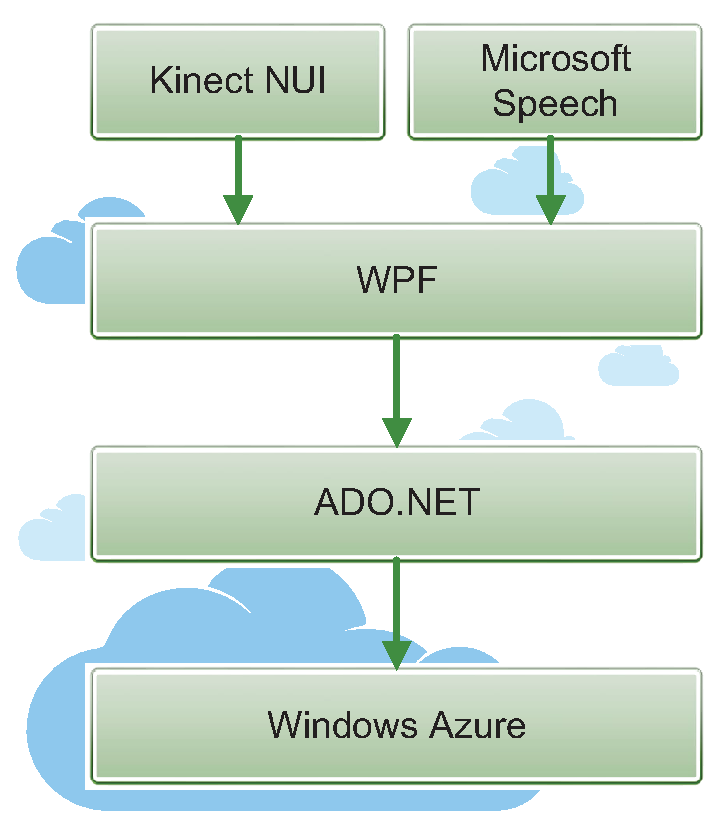
\includegraphics[width=0.8\linewidth]{ArchK}
\end{figure}

\end{multicols}

\end{document}